A Gaussian process (GP) is a collection of random variables, any finite number
of which have a joint Gaussian distribution \citep[e.g.,][]{rasmussen06}. A GP
can be used to define a distribution over functions $f(x) \sim \GP(\,\mu
(x)\,,\,k(x, x'))$, where each function value is a random variable indexed by $x
\in \BBR^d$, and $\mu\Colon \BBR^d \mathbin{\rightarrow} \BBR$ and $k\Colon
\BBR^d \times\BBR^d\mathbin{\rightarrow} \BBR$ are the mean and covariance
functions of the process.

Two popular covariance kernels are the RBF kernel
\begin{equation}\label{eqn:kernel_rbf}
  k_{\text{RBF}}(x, x') = s_f^2 \exp\left(\frac{\norm{x-x'}^2}{2\ell^2}\right)
\end{equation}
and the Mat\'ern kernel
\begin{equation}\label{eqn:kernel_matern}
  k_{\text{Mat},{\nu}}(x,x') =  s_f^2\frac{2^{1-\nu}}{\Gamma(\nu)} \left(
  \sqrt{2\nu}\frac{\norm{x-x'}}{\ell}\right)^\nu K_\nu\left(\sqrt{2\nu}
  \frac{\norm{x-x'}}{\ell}\right)
\end{equation}
where $1/2$, $3/2$, and $5/2$ are popular choices for $\nu$ to model 
heavy\hyp{}tailed correlations between function values. The spectral behavior of
these and other kernels has been well\hyp{}studied for years, and we recommend
\citep{wathen2015spectral} for recent results. Particularly relevant to our
discussion is a theorem due to Weyl, which says that if a symmetric kernel has
$\nu$ continuous derivatives, then the eigenvalues of the associated integral
operator decay like $\abs{\lambda_n} = \calo(n^{-\nu-1/2})$.  Hence, the
eigenvalues of kernel matrices for the smooth RBF kernel (and of any given
covariance matrix based on that kernel) tend to decay much more rapidly than
those of the less smooth Mat\'ern kernel, which has two derivatives at zero for
$\nu = 5/2$, one derivative at zero for $\nu = 3/2$, and no derivatives at zero
for $\nu = 1/2$.  This matters to the relative performance of Chebyshev and
Lanczos approximations of the log determinant for large values of $s_f$ and
small values of $\sigma$ on the exact and approximate RBF kernel. We also
introduce the spline kernel that we used in one of the experiments.
\begin{align}
  k_{\text{spline}}(x, y) = 
  \begin{cases}
    s^2 \big( \| x - y \|^3 + a\| x - y \|^2 + b \big) & d \text{ odd} \\
    s^2 \big( \| x - y \|^2\,\log \| x - y \| + a\| x - y \|^2 + b \big)  & d \text{ even}
  \end{cases}
\end{align}
where $a,b$ are chosen to make the spline kernel symmetric and positive definite
on the given domain. We denote any kernel hyper\hyp{}parameters by the vector
$\theta$. To be concise, we try to avoid explicitly denote the dependence of $k$
and associated matrices on $\theta$.

For any locations $X = \{x_1,\ldots,x_N\} \subset \BBR^d$, $f_X \Sim \calN
(\mu_X, \K{XX})$ where $f_X$ and $\mu_X$ represent the vectors of function
values for $f$ and $\mu$ evaluated at each of the $x_i \In X$, and $\K{XX}$ is
the matrix whose $(i,j)$ entry is $k(x_i, x_j)$. Suppose we have a vector of
corresponding function values $y \In \BBR^N$, where each entry is contaminated
by independent Gaussian noise with variance $\sigma^2$. Under a Gaussian process
prior depending on the covariance hyper\hyp{}parameters $\theta$, the log
marginal likelihood is given by
\begin{equation}\label{eqn:mloglik}
  \calL(\theta|y) = -\frac{1}{2}\left[(y-\mu_X)^T\alpha + \log\abs{\Ktil{XX}}
  + N\log 2\pi\right]\,,
\end{equation}
where $\alpha = \Ktil{XX}^{-1}(y-\mu_X)$ and $\Ktil{XX} = \K{XX} +\sigma^2I$.
Optimization of (\ref{eqn:mloglik}) is expensive, since the cheapest way of
evaluating $\log\abs{\Ktil{XX}}$ and its derivatives without taking advantage
of the structure of $\Ktil{XX}$ involves computing the $\calO(N^3)$ Cholesky
factorization of $\Ktil{XX}$. $\calO(N^3)$ computations is too expensive for
inference and learning beyond even just a few thousand points.

Meanwhile, differentiation is a linear operator, and (assuming a 
twice\hyp{}differentiable kernel) we may define a multi\hyp{}output GP for the
function and (scaled) gradient values with mean and kernel functions
\begin{equation}\label{eqn:meankernelderiv}
  \mu^{\nabla}(x) =
  \begin{bmatrix}
    \mu(x) \\ \dx_x \mu(x)
  \end{bmatrix}\,, \qquad
  k^{\nabla}(x,x') =
  \begin{bmatrix}
    k(x,x') & \left( \dx_{x'} k(x,x') \right)^T \\
    \dx_x k(x,x') & \ddx k(x,x')
  \end{bmatrix}\,,
\end{equation}
where $\dx_x k(x,x')$ and $\ddx k(x,x')$ represent the column vector of 
(scaled) partial derivatives in $x$ and the matrix of (scaled) second partials
in $x$ and $x'$, respectively. Scaling derivatives by a natural length scale
gives the multi\hyp{}output GP consistent units, and lets us understand
approximation error without weighted norms. As in the scalar GP case, we model
measurements of the function as contaminated by independent Gaussian noise.

Because the kernel matrix for the GP on function values alone is a submatrix
of the kernel matrix for function values and derivatives together, the
predictive variance in the presence of derivative information will be strictly
less than the predictive variance without derivatives. Hence, convergence of
regression with derivatives is always superior to convergence of regression
without, which is well\hyp{}studied in,~e.g.~\cite[Chapter 7]{rasmussen06}. 
\cref{fig:branin} illustrates the value of derivative information; fitting with
derivatives is evidently much more accurate than fitting function values alone.
In higher-dimensional problems, derivative information is even more valuable,
but it comes at a cost: the kernel matrix $K^{\nabla}_{XX}$ is of size $N
(d+1)$\hyp{}by\hyp{}$N(d+1)$. Scalable approximate solvers are therefore vital
in order to use GPs for large datasets with derivative data, particularly in
high\hyp{}dimensional spaces.

\begin{figure}[ht]
  \begin{center}
    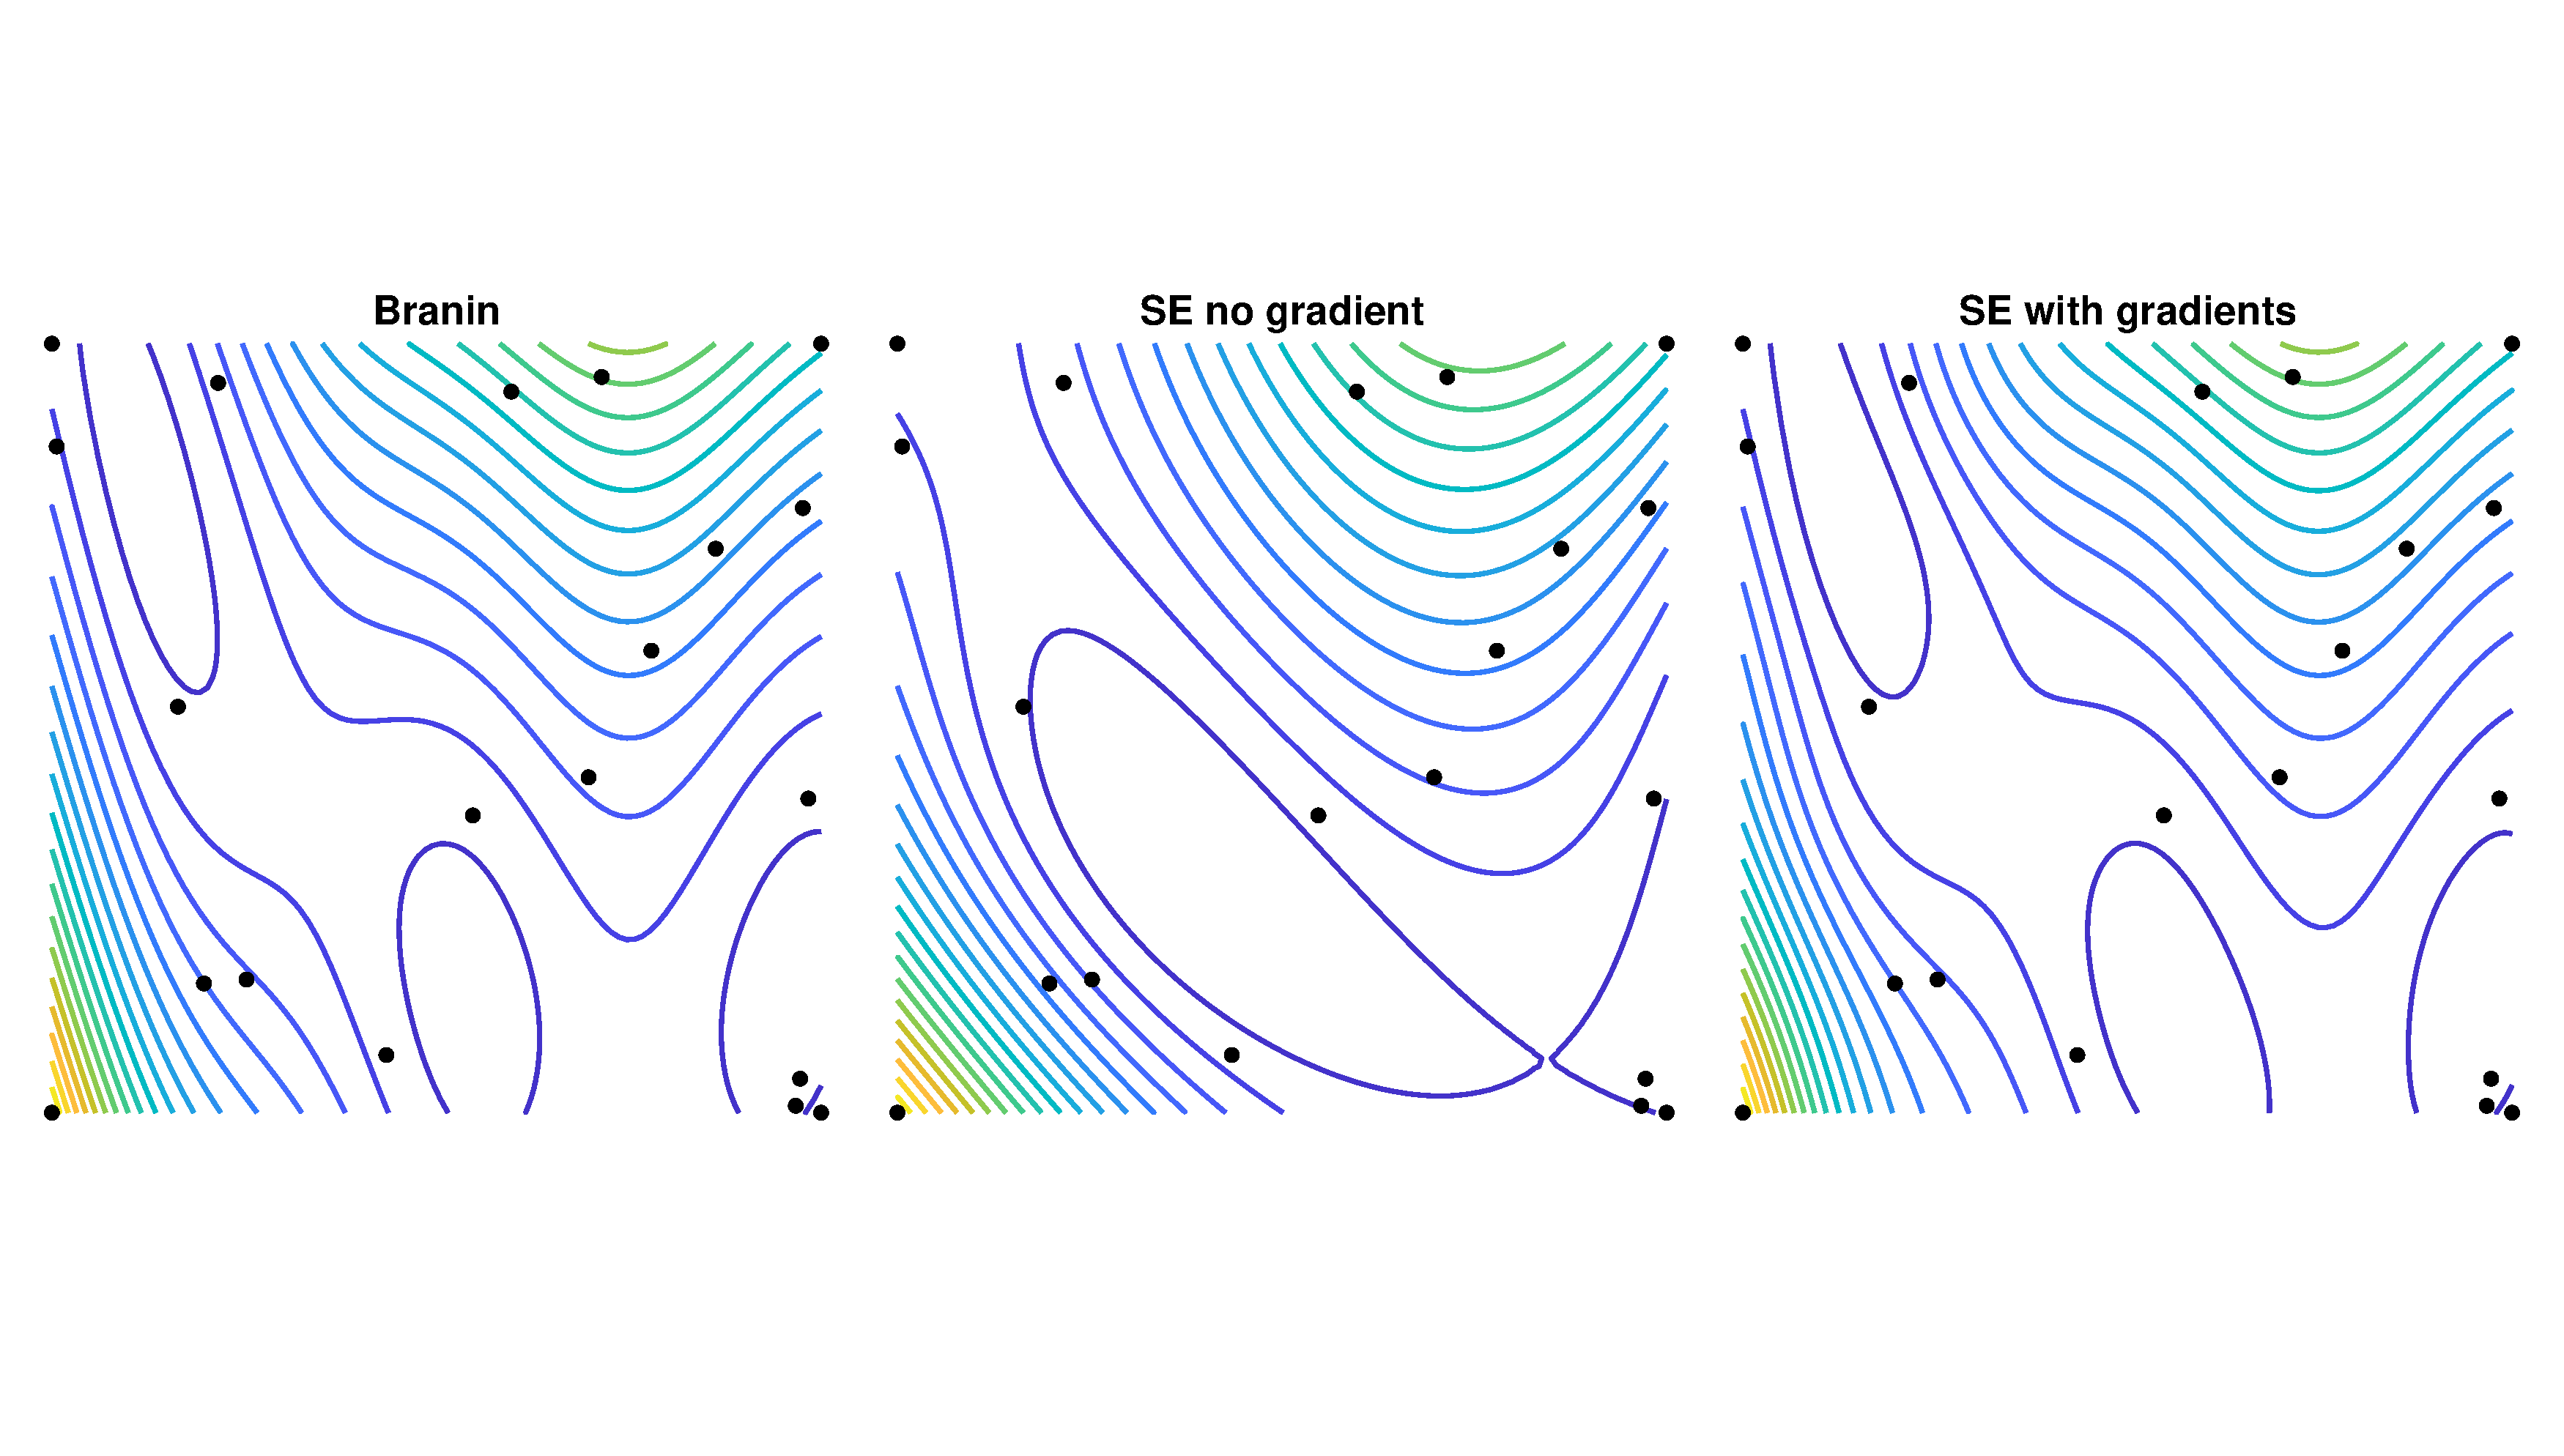
\includegraphics[width=\textwidth]{./sgpd/pics/branin}
    \caption{An example where gradient information pays off; the true function
    is on the left. Compare the regular GP without derivatives (middle) to the
    GP with derivatives (right). Unlike the former, the latter is able to
    accurately capture critical points of the function.}\label{fig:branin}
  \end{center}
\end{figure}

A popular approach to GP scalability is to replace the exact kernel $k(x, z)$
by an approximate kernel that admits fast computations 
\cite{quinonero2005unifying}. Several methods approximate $k(x, z)$ via {\em
inducing points} $U = \{u_j\}_{j=1}^M \binsubset \BBR^d$. An example is the
subset of regressor (SoR) kernel:
\begin{equation}\label{eqn:SoR}
  k^{\SoR}(x, z) = \K{xU}\K{UU}^{-1}\K{Uz}\,,
\end{equation}
which is a low\hyp{}rank approximation \cite{silverman1985some}. The SoR matrix
$\Ktil{XX}^{\SoR} \In \BBR^{N \times N}$ has rank at most $M$, allowing us to
solve linear systems involving $\Ktil{XX}^{\SoR} = \K{XX}^{\SoR} + \sigma^2I$
and to compute $\log\abs{\Ktil{XX}^{\SoR}}$ in $\calO(M^2 N + M^3)$ time.
Another popular kernel approximation is the fully independent training
conditional (FITC), which is a diagonal correction of SoR so that the diagonal
is the same as for the original kernel \cite{snelson2006sparse}.  Thus kernel
matrices from FITC have low\hyp{}rank plus diagonal structure. This modification
has had exceptional practical significance, leading to improved point
predictions and much more realistic predictive uncertainty 
\cite{quinonero2005unifying,quinonero2007}, making FITC arguably the most
popular approach for scalable Gaussian processes.

\citet{wilson2015kernel} provides a mechanism for fast MVMs through proposing
the structured kernel interpolation (SKI) approximation,
\begin{equation}\label{eqn:ski}
  \K{XX} \approx W \K{UU} W^{T}\,,
\end{equation}
where $W$ is an $N$\hyp{}by\hyp{}$M$ matrix of interpolation weights; the
authors of~\cite{wilson2015kernel} use local cubic interpolation so that $W$ is
sparse. The sparsity in $W$ makes it possible to naturally exploit algebraic
structure (such as Kronecker or Toeplitz structure) in $\K{UU}$ when the
inducing points $U$ are on a grid, for extremely fast matrix vector
multiplications with the approximate $\K{XX}$ even if the data inputs $X$ are
arbitrarily located. For instance, if $\K{UU}$ is Toeplitz, then each MVM with
the approximate $\K{XX}$ costs only $\calO(N + M \log M)$. By contrast, placing
the inducing points $U$ on a grid for classical inducing point methods, such as
SoR or FITC, does not result in substantial performance gains, due to the costly
cross-covariance matrices $\K{xU}$ and $\K{Uz}$. A limitation of SKI is that the
number of grid points increases exponentially with the dimension. This
exponential scaling has been addressed by structured kernel interpolation for
products (SKIP) \citep{gardner2018product}, which decomposes the kernel matrix
for a product kernel in $d$\hyp{}dimensions as a Hadamard (elemen\hyp{}wise)
product of one\hyp{}dimensional kernel matrices.